\newcommand{\Rplus}{\ensuremath{\nR_+}}
\newcommand{\Rnullplus}{\ensuremath{\nR^+_0}}

\subsection{Ressourcenverbrauch, Abängigkeit von n, Best- Worst- und Average-Case}
\begin{frame}{Laufzeit}
\centering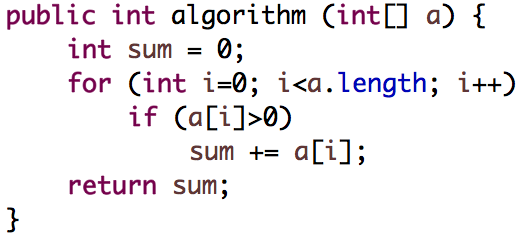
\includegraphics[height=4cm]{algorithm}

\begin{exampleblock}{Aufgabe}
	Wie viele \emph{Instruktionen} werden aufgerufen? \\% Worst-Case: n+1, Best-Case: 1, Average Case ?
	\pause
	Im \emph{worst case}? Im \emph{best case}? Im \emph{average case}?
\end{exampleblock}
\end{frame}

\subsection{O-Kalkül}
\begin{frame}{O-Notation}
	\begin{block}{Def. Asymptotisches Wachstum $\asymp$}
		Seien $f,g \from \nN_0 \to \Rnullplus$. Dann gilt
		\[
			f \asymp g \Leftrightarrow \exists c,c'\in \Rplus: \exists n_0\in \nN_0: \forall n\geq n_0: c f(n) \leq g(n) \leq c' f(n)
		\]
		Man sagt auch $g$ wächst genauso schnell wie $f$. $\asymp$ ist eine Äquivalenzrelation.
	\end{block}

	\begin{exampleblock}{Beispiele}
		\begin{itemize}
			\item $42n^6-33n^3+222n^2 -15 \asymp 66n^6+55555n^5$
			\item $n^{3}+5n^2 + 1\asymp 3n^3-n$
		\end{itemize}
	\end{exampleblock}
\end{frame}

\begin{frame}{$O$-Notation}
    \begin{block}{$\Theta$-Kalkül}
    	\begin{align*}
  			\Theta(f) &= \{ g \mid f \asymp g \} \\
  				   &= \{ g \mid \exists c,c'\in \Rplus: \exists n_0\in \nN_0: \forall  n\geq n_0: c f(n) \leq g(n) \leq c' f(n) \} 
		\end{align*}
    \end{block}

    \begin{exampleblock}{Bemerkungen}
    	\begin{itemize}
    		\item Im $\Theta$-Kalkül von $f(n)$ sind genau die Funktionen enthalten, die asymptotisch gleich schnell wachsen wie $f(n)$.
    		\item Schreibe $g(n) \in \Theta(f(n))$, wenn $g(n)$ asymptotisch gleichschnell wächst wie $f(n)$.
    		\item Ist $f$ ein Polynom, so sind insbesondere in $\Theta(f(n))$ alle Polynome enthalten, die den gleichen Grad wie $f$ haben.
    		\item Es gilt $\log_b(n) \in\Theta(\log_a(n))$. Die Basis ist also egal und man kann auch $\Theta(\log n)$ schreiben. % TODO Aufgabe und Beweis hierzu
    		% TODO Theta ist != Average Case
    	\end{itemize}
    \end{exampleblock}
\end{frame}

\begin{frame}{$O$-Notation}
    \begin{block}{Def.: $O$-Kalkül}
    	\[
    		O(f) = \{ g \mid \exists c\in \Rplus:\exists n_0\in\nN_0: \forall n\geq n_0: g(n) \leq c f(n)\}
    	\]

    	$g(n) \in O(f(n))$ (oder $g \preceq f$) genau dann, wenn $g$ asymptotisch höchstens so schnell wächst wie $f$.
    \end{block}
\pause
    \begin{block}{Def.: $\Omega$-Kalkül}
    	\[
    		\Omega(f) = \{ g \mid \exists c\in \Rplus:\exists n_0\in\nN_0: \forall n\geq n_0: g(n) \geq c f(n)\}
    	\]
    	
    	$g(n) \in \Omega(f(n))$ (oder $g \succeq f$) genau dann, wenn $g$ asymptotisch mindestens so schnell wächst wie $f$.
    \end{block}
\pause
    Beobachtung: $\Theta(f) = O(f) \cap \Omega(f)$
\end{frame}

\begin{frame}{$O$-Notation}
	\begin{exampleblock}{Aufgabe}
		\begin{enumerate}
			\item Für welches $c \in \Rplus$ gilt $5n^4 \in O(n^c)$ bzw $5n^4 \in \Omega(n^c)$?
			\item Für welches $c \in \Rplus$ gilt $5n^4 \in O(c^n)$ bzw $5n^4 \in \Omega(c^n)$?
			\item Für welches $c \in \Rplus$ gilt $2^n \in O(c^n)$ bzw $2^n \in \Omega(c^n)$?
			\item Zeige oder widerlege: $n \in \Theta(\sqrt{n})$
		\end{enumerate}
	\end{exampleblock}
\pause
	\begin{block}{Lösung}
		\begin{enumerate}
			\item Es gilt: $\forall c \geq 4$ bzw. $\forall c \leq 4$.
			\item Es gilt: $\forall c > 1$ bzw. $\forall c \leq 1$.
			\item Es gilt: $\forall c \geq 2$ bzw. $\forall c \leq 2$.
			\item \small Annahme: Die Behauptung ist richtig.\\
				Dann gilt: $n \in O(\sqrt{n}) \wedge n \in \Omega(\sqrt{n})$, insbesondere $n \in \Omega(\sqrt{n})$.\\
				$\Rightarrow \exists c\in \Rplus:\exists n_0\in\nN_0: \forall n\geq n_0: n \leq c \sqrt{n} \Leftrightarrow \frac{n}{\sqrt{n}} \leq c \Leftrightarrow \sqrt{n} \leq c$. Widerspruch.
				
		\end{enumerate}
	\end{block}
\end{frame}

\begin{frame}{$O$-Notation}
    \begin{exampleblock}{Aufgabe}
    	Zeige oder widerlege:
    	\[
    		f(n) + g(n) \in O(g(f(n)))
    	\]
    \end{exampleblock}
\pause
	\begin{block}{Lösung}
		Die Behauptung stimmt nicht. Wähle z.B. $f(n) = n^2$ und $g(n) = \sqrt{n}$ und führe dies zu einem Widerspruch.
	\end{block}
\end{frame}

\begin{frame}{$O$-Notation} % TODO: Logarithmusregeln, Typische Abschätzungskette (1 < log n < sqrt(n) < n < n log n < n c (c>1) < c^n < n!)
    \begin{itemize}
    	\item $\Theta$ entspricht \emph{nicht} dem average case.
    	\item $O(1)$ bedeutet konstante Laufzeit
    	\item Beachtet den \emph{Trick} mit den Limites\footnote{Ich weiß nicht, ob ihr den als Beweis in der Klausur oder auf dem Blättern verwenden dürft. Zur Kontrolle sollte man ihn aber kennen.}
        \item Es gilt mit Konstante $c \in \Rplus$ mit $c>1$
        \[
            1 \preceq \log n \preceq \sqrt{n} \preceq n \preceq n \log n \preceq n^c \preceq c^n \preceq n!
        \]
        %\nachgucken https://martin-thoma.com/die-landau-symbole/
    \end{itemize}
\end{frame}

\subsection{Master-Theorem}
\begin{frame}{Mastertheorem}
    \textbf{Problemstellung:}\\[1cm]    
    Gegeben sei eine \emph{rekursiv} definierte Funktion $T$.\\
    Frage: Welche Laufzeit hat $T$?\\[1cm]
    Beispiel:
    \[
    	T(n) = 8 T \left(\frac{n}{2} \right) + 1000n^2
    \]
    \\[1cm]\centering$\Rightarrow$ \emph{Mastertheorem}
\end{frame}

\begin{frame}{Mastertheorem}
    \begin{block}{Def.: Mastertheorem}
    	Seien $a\geq 1$ und $b>1$ Konstanten, $f \from \nN \to \Rnullplus$ und $T(n)$ eine Laufzeitfunktion der Form
    	\[
			T = a T\left(\frac{n}{b}\right) + f 
		\]
		Dann gilt nach dem \textbf{Mastertheorem}:
		\begin{itemize}
			\item \textbf{Fall 1:} \\ Wenn $f \in O(n^{\log_b a -\varepsilon})$ für ein $\varepsilon>0$ ist, dann ist $T\in \Theta(n^{\log_b a})$.
			\item \textbf{Fall 2:} \\ Wenn $f \in \Theta(n^{\log_b a})$ ist, dann ist $T\in \Theta(n^{\log_b a}\log n)$.
			\item\textbf{Fall 3:} \\  Wenn $f \in \Omega(n^{\log_b a +\varepsilon})$ für ein $\varepsilon>0$ ist, und wenn es eine Konstante $d$ gibt mit $0<d<1$, so dass für alle hinreichend großen $n$ gilt $af\left(\frac{n}{b}\right)\leq d f(n)$, dann ist $T\in \Theta(f)$.
		\end{itemize}
    \end{block}
\end{frame}

\begin{frame}{Mastertheorem}
    \begin{exampleblock}{Beispiel zum 1. Fall}
    	Sei $T(n) = 8 T \left(\frac{n}{2} \right) + 1000n^2$.
    	\begin{itemize}
    		\item Aus der Formel lässt sich ablesen:\\
    			$a=8$, $b=2$, $f(n)=1000n^2$
    		\item $n^{\log_b a}$ bestimmen:\\
    			$\log_b a = \log_2 8 = 3 \Rightarrow n^{\log_b a} = n^3$
    		\item $n^{\log_b a}$ mit $f(n)$ vergleichen: $1000n^2 \in O(n^3-\varepsilon)$?\\
    			Ja, für $\varepsilon = 1$ gilt $1000n^2 \in O(n^2)$.
    		\item Mit dem Mastertheorem folgt:\\
    			$T(n) = \Theta(n^3)$
    	\end{itemize}
    \end{exampleblock}
\end{frame}


\begin{frame}{Mastertheorem}
    \begin{exampleblock}{Beispiel zum 2. Fall}
    	Sei $T(n) = 2 T \left(\frac{n}{2} \right) + 10n$.
    	\begin{itemize}
    		\item Aus der Formel lässt sich ablesen:\\
    			$a=2$, $b=2$, $f(n)=10n$
    		\item $n^{\log_b a}$ bestimmen:\\
    			$\log_b a = \log_2 2 = 1 \Rightarrow n^{\log_b a} = n^1$
    		\item $n^{\log_b a}$ mit $f(n)$ vergleichen: $10n \in \Theta(n)$?\\
    			Ja!
    		\item Mit dem Mastertheorem folgt:\\
    			$T(n) = \Theta(n \log n)$
    	\end{itemize}
    \end{exampleblock}
\end{frame}



\begin{frame}{Mastertheorem}
    \begin{exampleblock}{Beispiel zum 3. Fall}
    	Sei $T(n) = 2 T \left(\frac{n}{2} \right) + n^2$.
    	\begin{itemize}
    		\item Aus der Formel lässt sich ablesen:\\
    			$a=2$, $b=2$, $f(n)=n^2$
    		\item $n^{\log_b a}$ bestimmen:\\
    			$\log_b a = \log_2 2 = 1 \Rightarrow n^{\log_b a} = n^1$
    		\item $n^{\log_b a}$ mit $f(n)$ vergleichen: $n^2 \in \Omega(n^{1+\varepsilon})$?\\
    			Ja, für $\varepsilon = 1$ gilt $n^2 \in \Omega(n^2)$.
    		\item Zusatzbedingung überprüfen: Ist $af\left(\frac{n}{b}\right)\leq d f(n)$?\\
    			Ja, für $d = \frac{1}{2}$ gilt $\forall n \geq 1 \; : \; \frac{1}{2}n^2 \leq \frac{1}{2}n^2$
    		\item Mit dem Mastertheorem folgt:\\
    			$T(n) = \Theta(n^2)$
    	\end{itemize}
    \end{exampleblock}
\end{frame}